%%%%%%%%%%%%%%%%%%%%%%%%%%%%%%%%%%%%%%%%%
% Wenneker Article
% LaTeX Template
% Version 2.0 (28/2/17)
%
% This template was downloaded from:
% http://www.LaTeXTemplates.com
%
% Authors:
% Vel (vel@LaTeXTemplates.com)
% Frits Wenneker
%
% License:
% CC BY-NC-SA 3.0 (http://creativecommons.org/licenses/by-nc-sa/3.0/)
%
%%%%%%%%%%%%%%%%%%%%%%%%%%%%%%%%%%%%%%%%%

%----------------------------------------------------------------------------------------
%	PACKAGES AND OTHER DOCUMENT CONFIGURATIONS
%----------------------------------------------------------------------------------------

\documentclass[10pt, a4paper, twocolumn]{article}

%%%%%%%%%%%%%%%%%%%%%%%%%%%%%%%%%%%%%%%%%
% Wenneker Article
% Structure Specification File
% Version 1.0 (28/2/17)
%
% This file originates from:
% http://www.LaTeXTemplates.com
%
% Authors:
% Frits Wenneker
% Vel (vel@LaTeXTemplates.com)
%
% License:
% CC BY-NC-SA 3.0 (http://creativecommons.org/licenses/by-nc-sa/3.0/)
%
%%%%%%%%%%%%%%%%%%%%%%%%%%%%%%%%%%%%%%%%%

%----------------------------------------------------------------------------------------
%	PACKAGES AND OTHER DOCUMENT CONFIGURATIONS
%----------------------------------------------------------------------------------------

\usepackage[english]{babel} % English language hyphenation

\usepackage{microtype} % Better typography

\usepackage{amsmath,amsfonts,amsthm} % Math packages for equations

\usepackage[svgnames]{xcolor} % Enabling colors by their 'svgnames'

\usepackage[hang, small, labelfont=bf, up, textfont=it, position=below, skip=5pt]{caption} % Custom captions under/above tables and figures
\setlength{\belowcaptionskip}{-10pt}

\usepackage{booktabs} % Horizontal rules in tables

\usepackage{lastpage} % Used to determine the number of pages in the document (for "Page X of Total")

\usepackage{graphicx} % Required for adding images

\usepackage{enumitem} % Required for customising lists
\setlist{noitemsep} % Remove spacing between bullet/numbered list elements

\usepackage{sectsty} % Enables custom section titles
\allsectionsfont{\usefont{OT1}{phv}{b}{n}} % Change the font of all section commands (Helvetica)

\usepackage[pdfborder={0 0 0},colorlinks=true,linkcolor={black},citecolor={black},urlcolor={blue!60!black}]{hyperref}

%----------------------------------------------------------------------------------------
%	MARGINS AND SPACING
%----------------------------------------------------------------------------------------

\usepackage{geometry} % Required for adjusting page dimensions

\geometry{
	top=1cm, % Top margin
	bottom=1.5cm, % Bottom margin
	left=2cm, % Left margin
	right=2cm, % Right margin
	includehead, % Include space for a header
	includefoot, % Include space for a footer
	%showframe, % Uncomment to show how the type block is set on the page
}

\setlength{\columnsep}{7mm} % Column separation width

%----------------------------------------------------------------------------------------
%	FONTS
%----------------------------------------------------------------------------------------

\usepackage[T1]{fontenc} % Output font encoding for international characters
\usepackage[utf8]{inputenc} % Required for inputting international characters

\usepackage{XCharter} % Use the XCharter font

%----------------------------------------------------------------------------------------
%	HEADERS AND FOOTERS
%----------------------------------------------------------------------------------------

\usepackage{fancyhdr} % Needed to define custom headers/footers
\pagestyle{fancy} % Enables the custom headers/footers

\renewcommand{\headrulewidth}{0.0pt} % No header rule
\renewcommand{\footrulewidth}{0.4pt} % Thin footer rule

\renewcommand{\sectionmark}[1]{\markboth{#1}{}} % Removes the section number from the header when \leftmark is used

%\nouppercase\leftmark % Add this to one of the lines below if you want a section title in the header/footer

% Headers
\lhead{} % Left header
\chead{\textit{\thetitle}} % Center header - currently printing the article title
\rhead{} % Right header

% Footers
\lfoot{} % Left footer
\cfoot{} % Center footer
\rfoot{\footnotesize Page \thepage\ of \pageref{LastPage}} % Right footer, "Page 1 of 2"

\fancypagestyle{firstpage}{ % Page style for the first page with the title
	\fancyhf{}
	\renewcommand{\footrulewidth}{0pt} % Suppress footer rule
}

%----------------------------------------------------------------------------------------
%	TITLE SECTION
%----------------------------------------------------------------------------------------

\newcommand{\authorstyle}[1]{{\large\usefont{OT1}{phv}{b}{n}\color{DarkRed}#1}} % Authors style (Helvetica)

\newcommand{\institution}[1]{{\footnotesize\usefont{OT1}{phv}{m}{sl}\color{Black}#1}} % Institutions style (Helvetica)

\usepackage{titling} % Allows custom title configuration

\newcommand{\HorRule}{\color{DarkGoldenrod}\rule{\linewidth}{1pt}} % Defines the gold horizontal rule around the title

\pretitle{
	\vspace{-30pt} % Move the entire title section up
	\HorRule\vspace{10pt} % Horizontal rule before the title
	\fontsize{32}{36}\usefont{OT1}{phv}{b}{n}\selectfont % Helvetica
	\color{DarkRed} % Text colour for the title and author(s)
}

\posttitle{\par\vskip 15pt} % Whitespace under the title

\preauthor{} % Anything that will appear before \author is printed

\postauthor{ % Anything that will appear after \author is printed
	\vspace{10pt} % Space before the rule
	\par\HorRule % Horizontal rule after the title
	\vspace{20pt} % Space after the title section
}

%----------------------------------------------------------------------------------------
%	ABSTRACT
%----------------------------------------------------------------------------------------

\usepackage{lettrine} % Package to accentuate the first letter of the text (lettrine)
\usepackage{fix-cm}	% Fixes the height of the lettrine

\newcommand{\initial}[1]{ % Defines the command and style for the lettrine
	\lettrine[lines=3,findent=4pt,nindent=0pt]{% Lettrine takes up 3 lines, the text to the right of it is indented 4pt and further indenting of lines 2+ is stopped
		\color{DarkGoldenrod}% Lettrine colour
		{#1}% The letter
	}{}%
}

\usepackage{xstring} % Required for string manipulation

\newcommand{\lettrineabstract}[1]{
	\StrLeft{#1}{1}[\firstletter] % Capture the first letter of the abstract for the lettrine
	\initial{\firstletter}\textbf{\StrGobbleLeft{#1}{1}} % Print the abstract with the first letter as a lettrine and the rest in bold
} % Specifies the document structure and loads requires packages

%----------------------------------------------------------------------------------------
%	ARTICLE INFORMATION
%----------------------------------------------------------------------------------------

\title{My favorite physicist is FERMI} % The article title

\author{
	\authorstyle{Group for Lasers and Plasmas\textsuperscript{$\ast,\dagger,\ddagger$}} % Authors
	\newline\newline % Space before institutions
	\textsuperscript{$\ast$}\institution{Institute for Plasmas and Nuclear Fusion}\\
	\textsuperscript{$\dagger$}\institution{Instituto Superior Técnico, Lisboa}\\
	\textsuperscript{$\ddagger$}\institution{\url{http://epp.ist.utl.pt/}}
}


\date{May 5, 2017}
%----------------------------------------------------------------------------------------


\begin{document}

\maketitle % Print the title

\thispagestyle{firstpage} % Apply the page style for the first page (no headers and footers)

%----------------------------------------------------------------------------------------
%	ABSTRACT
%----------------------------------------------------------------------------------------

\lettrineabstract{This is a small example of a showcase for a session on git/github. The main idea is to use some resources available only and add a section of one famous physicist. You can even use pictures of equations or something you associate with this person. It does not matter for now. Just use some reference if you are copying something. Everyone likes to be acknowledged.}

%----------------------------------------------------------------------------------------
%	ARTICLE CONTENTS
%----------------------------------------------------------------------------------------
\section*{Instructions for authors}

A description on how to work with the repository can be found on \href{https://github.com/ahelm/my-favorite-physicist}{github}. Below you can find an example how to add one physicist you like to this document. You can use images or equations inside the document, but if you take some text from an online resource be so kind and provide where you have taken it from.

The directory structure is designed to reduce conflicts and create a better overview. The directory \texttt{/content} includes the different \texttt{.tex} files and you should add the corresponding \LaTeX\ files over there. Please store the images in the folder \texttt{content/figures}.

\section*{Albert Einstein\protect\footnote{\url{https://en.wikipedia.org/wiki/Albert_Einstein}}}

\begin{figure}[ht]
  \centering
  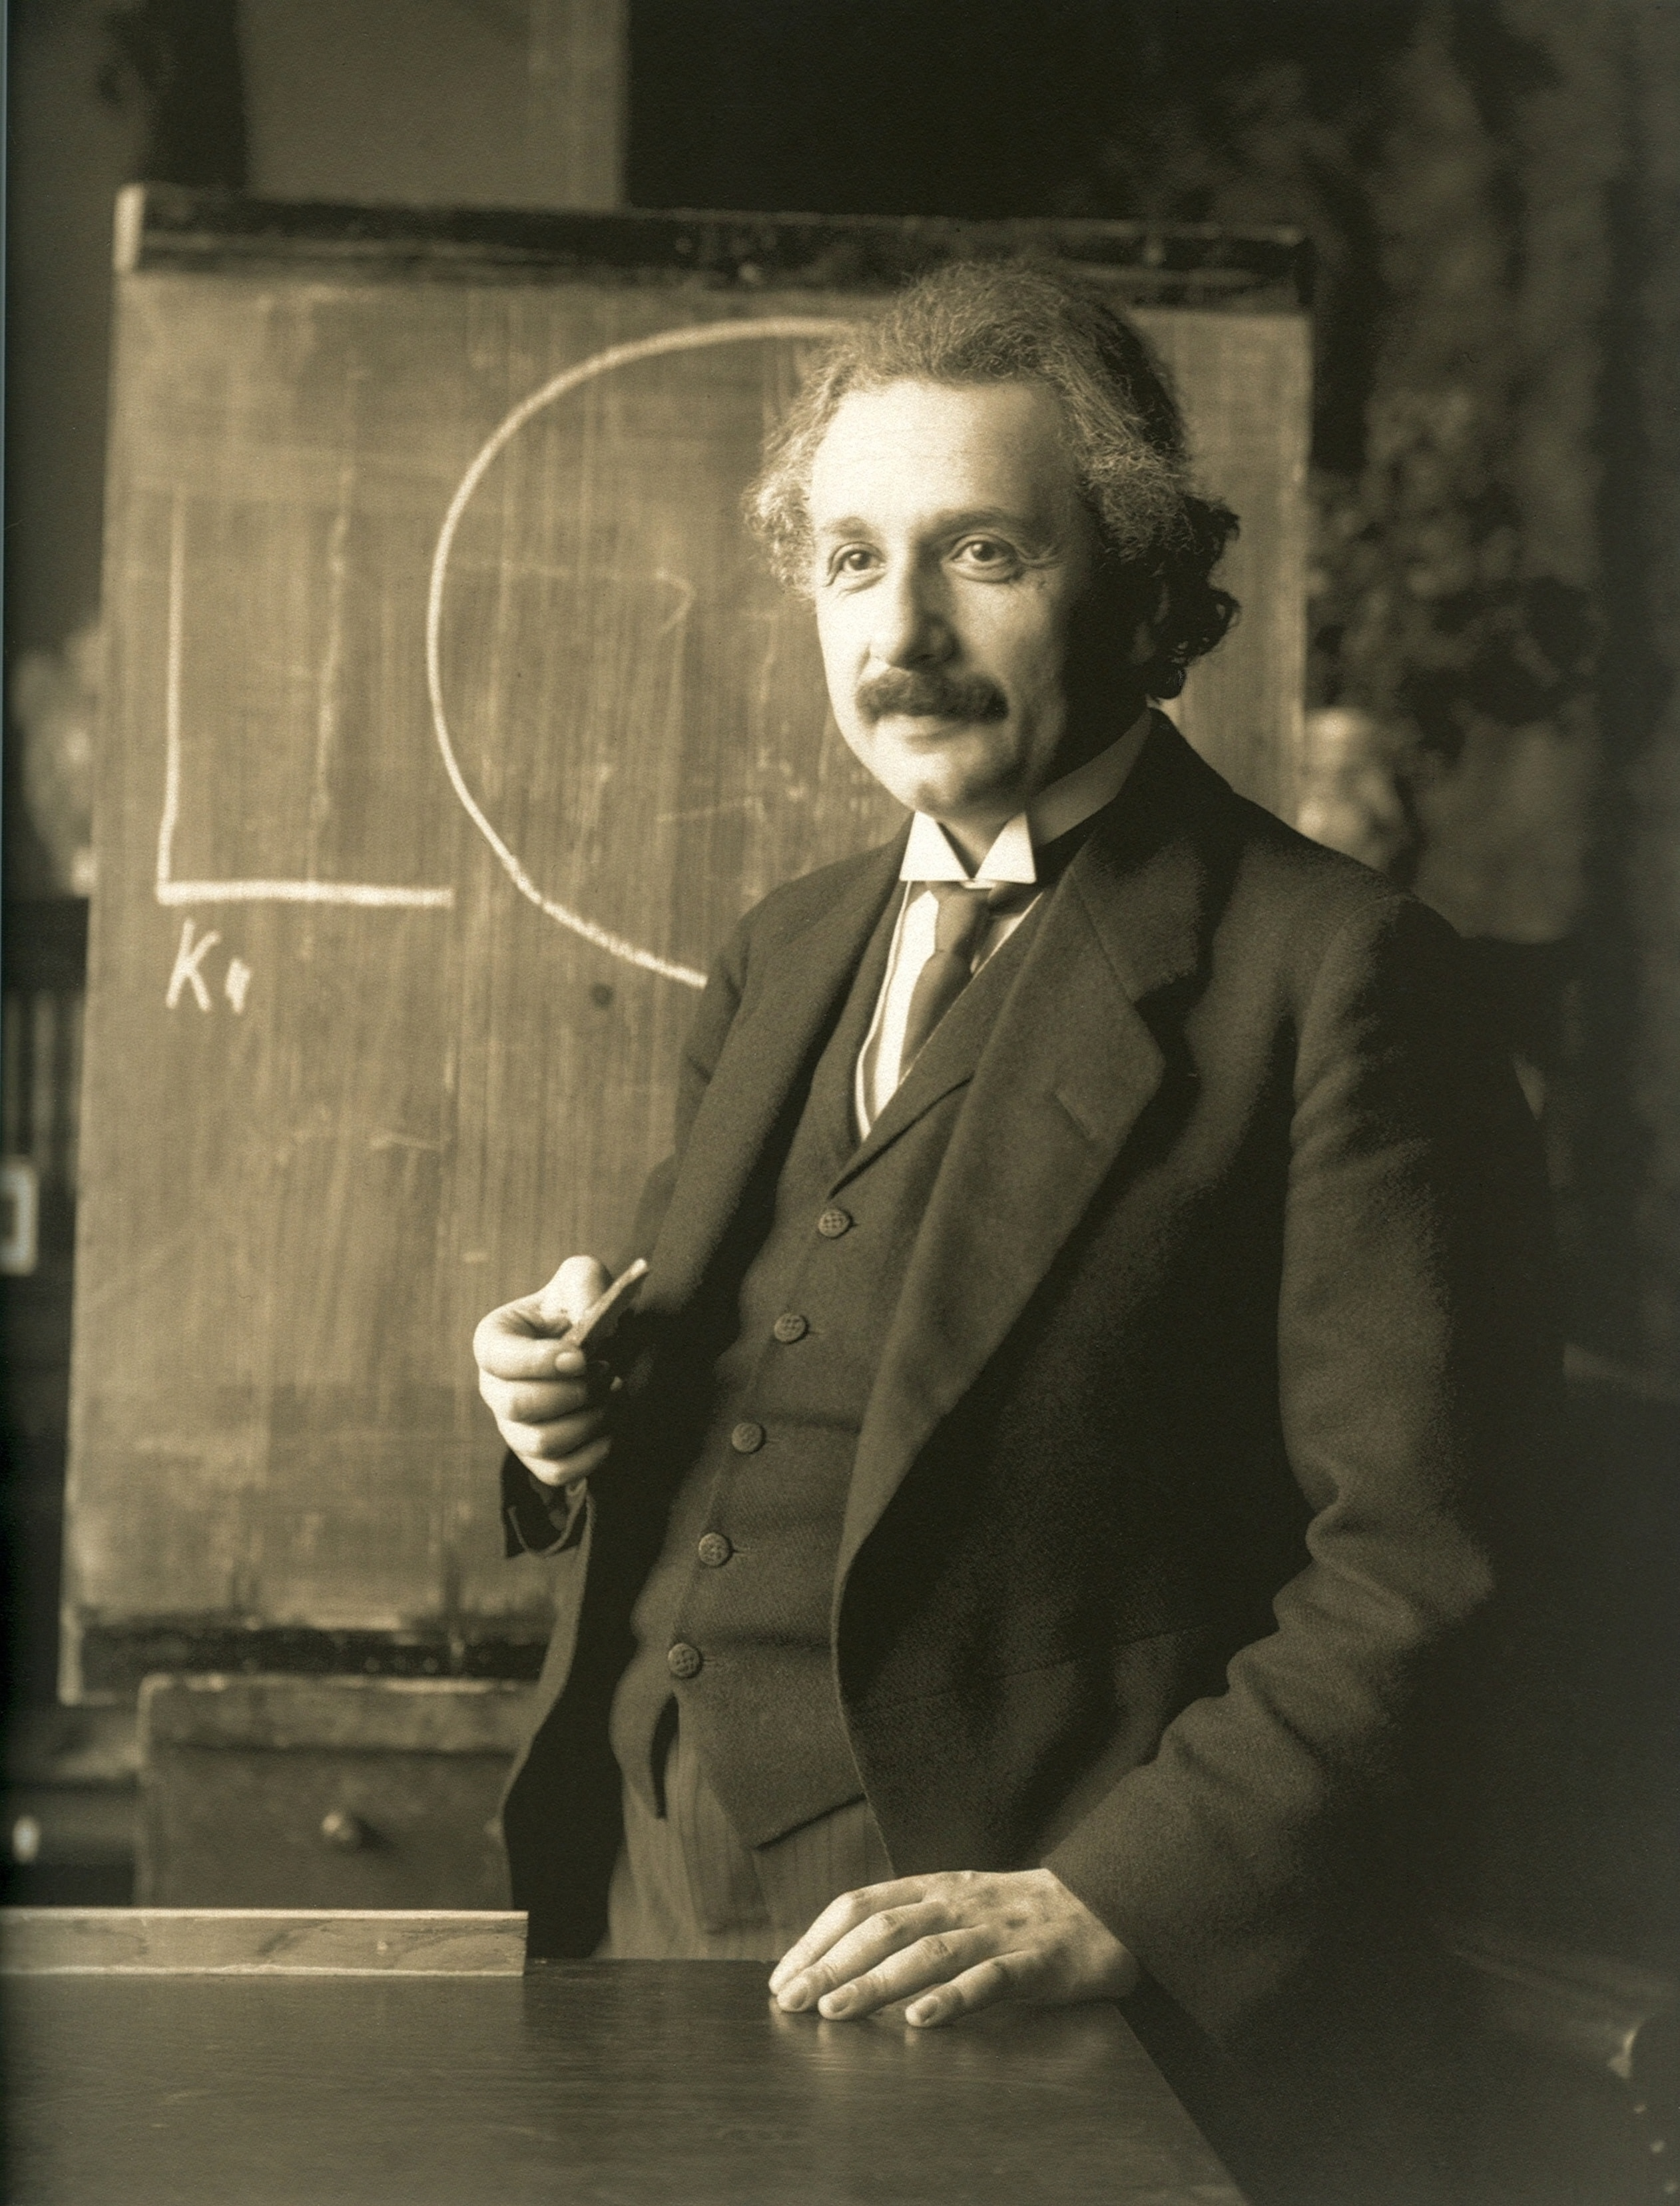
\includegraphics[width=0.8\linewidth]{content/figures/albert_einstein_picuture.jpg}
  \caption{Albert Einstein in 1921\protect\footnotemark}
\end{figure}
\footnotetext{\url{https://commons.wikimedia.org/wiki/File:Einstein_1921_by_F_Schmutzer_-_restoration.jpg}}

Albert Einstein (14 March 1879 – 18 April 1955) was a German-born theoretical physicist. He developed the theory of relativity, one of the two pillars of modern physics (alongside quantum mechanics). Einstein's work is also known for its influence on the philosophy of science. Einstein is best known in popular culture for his mass–energy equivalence formula $E = mc^2$ (which has been dubbed ``the world's most famous equation''). He received the 1921 Nobel Prize in Physics ``for his services to theoretical physics, and especially for his discovery of the law of the photoelectric effect'', a pivotal step in the evolution of quantum theory.

Near the beginning of his career, Einstein thought that Newtonian mechanics was no longer enough to reconcile the laws of classical mechanics with the laws of the electromagnetic field. This led him to develop his special theory of relativity during his time at the Swiss Patent Office in Bern (1902–1909), Switzerland. He realized, however, that the principle of relativity could also be extended to gravitational fields, and with his subsequent theory of gravitation in 1916, he published a paper on general relativity. He continued to deal with problems of statistical mechanics and quantum theory, which led to his explanations of particle theory and the motion of molecules. He also investigated the thermal properties of light which laid the foundation of the photon theory of light. In 1917, Einstein applied the general theory of relativity to model the large-scale structure of the universe.

Between 1895 and 1914 he lived in Switzerland (except for one year in Prague, 1911–12), where he received his academic diploma from the Swiss Federal Polytechnic in Zürich (later the Eidgenössische Technische Hochschule, ETH) in 1900. He later taught there at the same institute as a professor of theoretical physics between 1912 and 1914 before he left for Berlin. In 1901, after being stateless for more than five years, Einstein acquired Swiss citizenship, which he kept for the rest of his life. In 1905, Einstein was awarded a PhD by the University of Zürich. The same year, his annus mirabilis (miracle year), he published four groundbreaking papers, which were to bring him to the notice of the academic world, at the age of 26.

He was visiting the United States when Adolf Hitler came to power in 1933 and, being Jewish, did not go back to Germany, where he had been a professor at the Berlin Academy of Sciences. He settled in the United States, becoming an American citizen in 1940. On the eve of World War II, he endorsed a letter to President Franklin D. Roosevelt alerting him to the potential development of ``extremely powerful bombs of a new type'' and recommending that the U.S. begin similar research. This eventually led to what would become the Manhattan Project. Einstein supported defending the Allied forces, but generally denounced the idea of using the newly discovered nuclear fission as a weapon. Later, with the British philosopher Bertrand Russell, Einstein signed the Russell–Einstein Manifesto, which highlighted the danger of nuclear weapons. Einstein was affiliated with the Institute for Advanced Study in Princeton, New Jersey, until his death in 1955.

Einstein published more than 300 scientific papers along with over 150 non-scientific works. On 5 December 2014, universities and archives announced the release of Einstein's papers, comprising more than 30,000 unique documents. Einstein's intellectual achievements and originality have made the word ``Einstein'' synonymous with ``genius''.


\end{document}
